% used template from Overleaf: https://www.overleaf.com/latex/templates/academic-paper/rjttmshldvgg

% weird fix for biblatex from: https://tex.stackexchange.com/questions/568021/package-biblatex-error-patching-addtocontents-failed
\let\latexaddtocontents\addtocontents
\documentclass[10pt]{paper}
\let\addtocontents\latexaddtocontents



\usepackage{amssymb}
\usepackage{amsmath}
\usepackage{graphicx}
\usepackage{dcolumn}
\usepackage{hyperref}
\usepackage{float}

\graphicspath{ {./images/} }

\usepackage{biblatex} % https://www.overleaf.com/learn/latex/Bibliography_management_in_LaTeX
\addbibresource{main.bib}

% Code blocks
\usepackage[theme=default]{jlcode}
% \usepackage{listings, xcolor}

% \definecolor{codegreen}{rgb}{0,0.6,0}
% \definecolor{codegray}{rgb}{0.5,0.5,0.5}
% \definecolor{codepurple}{rgb}{0.58,0,0.82}
% \definecolor{backcolour}{rgb}{0.95,0.95,1}

% \lstdefinestyle{mystyle}{
%     backgroundcolor=\color{backcolour},   
%     commentstyle=\color{codegreen},
%     keywordstyle=\color{magenta},
%     numberstyle=\tiny\color{codegray},
%     stringstyle=\color{codepurple},
%     basicstyle=\ttfamily\footnotesize,
%     breakatwhitespace=false,         
%     breaklines=true,                 
%     captionpos=b,                    
%     keepspaces=true,                 
%     numbers=left,                    
%     numbersep=5pt,                  
%     showspaces=false,                
%     showstringspaces=false,
%     showtabs=false,                  
%     tabsize=4
% }

% \lstset{style=mystyle}

\begin{document}

\title{MATH181 Project: Automatic Identification of Nonlinear Systems}
\author{Theo Rode}

% \affiliation{Somewhere}

% \begin{abstract}
% Your abstract.
% \end{abstract}

\maketitle

\section{Introduction} \label{sec:introduction}
Dynamical systems are mathematical objects used to describe anything and everything that changes. This gives rise to their utility in modeling a vast array of applications. Of course, physical systems are of particular interest as the rules of physics work in terms of velocity and acceleration---the descriptors of movement. 
Though, in principle, far more than the cannonical examples of physical movement are ``changing.'' Economic models describe the changes in producer and consumer supply and demand, while biologists model the rise and fall of organism populations in an ecosystem. 
The prevalence of these inherently changing systems leads to the field of dynamical systems having vast applicability to the world of mathematical modeling. Though while they are often the natural language to describe these situations, determining the particular dynamics in a given system is a fundamentally difficult problem. 

This paper discusses a method through which data can be used to uncover the governing equations for a dynamical system. 
%
% This project discusses the procedure of recovering the underlying equations for the dynamics given noisy data collected by the system. So called ``physics-inspired'' or ``physics-informed'' AI.
% The goal of this field is to gain a physical understanding of systems where we can measure various trajectories, but the dynamics are unknown. Though this is additionally useful in situations where complex systems have dynamical properties that can be modeled on a smaller scale. 
In particular, the focus of this paper is on discussing the results demonstrated by Steven Brunton, Joshua Proctor, and Nathan Kutz in their paper published in 2016. They propose a new algorithm for reconstructing dynamics within a system called SINDy (Sparse Identification of Nonlinear Dynamics) \cite{sindy}.
% This first section aims to discuss the field more broadly and relevant papers to the results proposed in the aforementioned paper as well as more generally in the field. 
In this first section, I will discuss the field more broadly prior to Brunton, Proctor, and Kutz published their work. This will include a dicussion of relevant papers that provided the groundwork for the SINDy algorithm.
In the section section (\ref{sec:mathematical_background}), I will discuss the relevant mathematical background for SINDy and its underlying mathematics. Section \ref{sec:results} will go deeper into the results demonstrated by Brunton et al. by discussing my work to recreate the SINDy algorithm. 
Finally, section \ref{sec:discussion} offers a dicussion of the results in the paper and further areas of interest. 

The authors of \cite{sindy} give two foundational papers for recovering the dynamics of nonlinear systems: a paper by Josh Bongard and Hod Lipson \cite{bongard} and one by Michael Schmidt and Hod Lipson \cite{schmidt}, in 2007 and 2009 respectively.
Bongard and Lipson \cite{bongard} outline a method for ``reverse engineering'' the dynamics of nonlinear systems by utilizing an active learning system. 
The main process of the algorithm is a technique labeled \textbf{symbolic regression}. Fundamentally, symbolic regression is a regression algorithm that is used to build up arbitrary equations to represent the given data. This is often accomplished through a genetic algorithm where ``function blocks'' are used to build possible functions, which are then tested with the best being used to create the next generation.
In \cite{bongard}, symbolic regression is made usable for complicated (nonlinear) systems by introducing three concepts: partitioning, automated probing, and snipping. Partitioning is a process by which the algorithm is able to model each of the variables in the system separately using stochastic optimization. 
Each of the variables are integrated by substituting in representations of the other variables rather than integrating the variables together. This method significantly reduces the overhead when working with high dimensional systems. Automated probing allows the algorithm to explore the system through active learning. After candidate models are created, the algorithm attempts to create many ``tests'' which are judged against their ability to disprove as many of the candidate models as possible. Then, the test which rejects as many of the candidate models as possible is used to judge the performance of all candidate models in order to pick the most capable ones. From this, the next generation of candidate models can be generated. 
Finally, snipping is a process to reduce the complexity of the generated models and prevent over-fitting. In particular, when creating another generation of models, occasionally certain subexpressions will be replaced with a value of the subexpression picked uniformly from its range. 
This process reduces situations where the model constructs complex subexpressions which take on narrow ranges of values, a hallmark of over-fitting data.
Together, these innovations on the process of symbolic regression allowed Bongard and Lipson to create a framework that was applicable to an array of real-world systems. The framework demonstrated the ability to find nonlinearities and interdependencies as well as an ability to scale successfully. However, the authors note that current limitations include not yet demonstrating scalability to much larger biological models and an inability to work on data where certain variables are unobservable, as a key component of the framework was the active learning \cite{bongard}. 

Schmidt and Lipson present another algorithm for reconstructing dynamics, also based on \textbf{symbolic regression} \cite{schmidt}. 
This paper focuses on presenting a new metric for comparing the accuracy of various candidate equations in order to better search for invariants within the system. 
In particular, once candidate equations are generated (initially randomly from a set of ``building blocks''), the partial derivative pairings of every pair of variables are compared to the numerically calculated 
partial derivative pairings in order to select the equations which model these pairs the closest. They generate the next generation of equations probablistically from the best equations.
To determine the accuracy of equations on the observed data, the authors withhold a random sample from the collected data for testing and when the equations reach a certain level of accuracy, the algorithm terminates.
Finally, equations are prioritized accoriding to measured parsimony---roughly calculated as the number of terms in the expression. 
The authors were able to demonstrate that this algorithm could reconstruct invariants from numerous physical systems effectively. Additionally, they noticed that with a limited set of building blocks, the algorithm found approximations to functions like sines and cosines, utilizing the available building blocks, when such functions were part of the physical invariant \cite{schmidt}. 

% TALK ABOUT MORE RECENT PAPER? 

% mention LASSO: https://watermark.silverchair.com/jrsssb_58_1_267.pdf?token=AQECAHi208BE49Ooan9kkhW_Ercy7Dm3ZL_9Cf3qfKAc485ysgAAA3swggN3BgkqhkiG9w0BBwagggNoMIIDZAIBADCCA10GCSqGSIb3DQEHATAeBglghkgBZQMEAS4wEQQMUUUguuXeXSXLKrHyAgEQgIIDLjjGy45TLem5-SWBsiKqth_ATlBiN1U8oB2jwRawwKAQLhSBq9mr6Xxoy5NWpIW4ICk-qvgW4vlMPUFgp3aXI1CPO7BCP5VER8ruRsVHe-xFxsJrz1Idh0wPazgvEt6cHJfNxeEWOxiBPBYyPMSESASwKHfX4EQxoq_Au2Bzkg6gFRWiGBSestTCekla3yBbmJ9FMWqtL0hVt0LtXXwf81ICM7qX_y4YW0ZKOUS2M9z2EEIMgWCkfeivpJT0CJi8CWfL7oorAsCpsu_wxGucDzNm_Ki_SqlaNZAU-mI3iVIxr4FUCWJxgh8mfeHxCJttaC1p97U5TX3OTzL_S71k4-4DNrWUaGhKgRe2QEXZg8SLWnsRolTN6MBmtlfstqIoMP4PPsaIJ_93YWxRALnL_pdknBTh2edgos_NVDt6nMC41LoCepoI8cSD0BgcJo3L_v3Fa4KOnVHpfLED7PCgj_mT7UY2d4dJlO_3ryWWXa_NhgGbXUywx8KOJzC0M1O0ZAEo0pmz50mMzp0XyVQX6sl3uCHzDB8zHWfI8-BHBzC5dYDHKeGx7xS8H4wws5EriZX_jeHIG4NYUTbCLV0IaVCx4nxTrc6gglm8D2aqlBjI52KHj7iIi78EKZ7pcrgfJ6-RA2rb2435a--KHrXE1S5E4feJA2KWhx7VBEn-t53uszHD7bE3sOrHU7qHDzYKWeuk3T_ewVJuyE8_-P7tLVtWoSKxvsqT1mR4inR6UKmJbHjyTH0HV2QQ6ybtztDj7hrgVPQROkmBMhURkCaGMJHTFeYtdF9W4ZGb7O432f22h7ousNc5dDIAAyGtxGI6doK4bS35eWPzqVMZ5Q4D9WIncF_ehYujzLdosbyNyZLt9SPwaPCBfHwwXCxyDkArH_MWjjOyz-h6D0JxXRyTOyZhw9vbNp8vkpccU0W1zNfmyYn8SkDQJwpN5L1mUpPXeASQb4eH8rE6VttkD09Lmqv4hy502xE-88dYoKVoOToavtAVT9nc-ARwnQ4eyS1dkmPBfy9KOlIz7WHvIg0XFbNoG5AoMjCya6vdfYmDLgNJuhvRVilIhFkuuxMw2cc
% supposedly helpful for sparse regression? 

% talk about advances in compressed sensing seen here: https://journals.aps.org/prl/pdf/10.1103/PhysRevLett.106.154101

\section{Mathematical Background} \label{sec:mathematical_background}
For the SINDy algorithm, the authors aimed to reframe the problem of recovering nonlinear dynamics using \textbf{sparse regression} and \textbf{compressed sensing} \cite{sindy}. Both sparse regression and compressed sensing broadly refer to the process of finding a regression solution to a problem such that the solution is sparse in some space \cite{sindy}. 
Brunton et al. relate that utilizing sparse regression is a strategy to reduce the noise present in the fitting of systems \cite{sindy}. The particular assumptions for sparse regression come from the idea that in most cases, the dynamics for a particular system will be governed by a small set of given basis functions. Therefore, the sparsity also gives advantages for computation as we can increase the size of the function space dramatically without needing significantly more computation \cite{sindy}. 

% mention LASSO here as alternative method for sparse regression
The authors of \cite{sindy} propose an iterative algorithm for sparse regression. In particular, they start with a least-squares fit to the data, and then iteratively remove coefficients below a given threshold. By refitting with the remaining, nonzero terms iteratively, the algorithm can arrive at a sparse solution \cite{sindy}. 

The SINDy algorithm relies on the availability of both sampled data, $\mathbf X$, and the sampled derivative, $\mathbf{\dot X}$. However, the authors note that the availability of derivative measurements are not guaranteed and therefore propose using the \textbf{total variation regularized derivative} to mitigate the noise created from numerically calculating $\mathbf {\dot X}$ from $\mathbf X$ \cite{sindy}. In particular, they cite the algorithm used by Rudin et al. \cite{rudin}. 
Here, Rudin et al. use a framework for computing a desired, denoised output, $u$, from a noisy input, $u_0$, by assuming that $u = u_0 + n$ for some white noise function $n$. It is assumed that $n$ has a mean of $0$ with some given standard deviation. 
The minmization problem corresponds to minimizing $\int_\Omega \sqrt{u_x^2 + u_y^2} \, \mathrm d A$, which is contrained by $\int_\Omega u \, \mathrm dA = \int_\Omega u_0 \, \mathrm dA$ under the assumption of the additive white noise. It is then proposed to solve for $u$ through either an iterative algorithm (i.e. simulated annealing) or, preferably, a PDE solver to find local minimum \cite{rudin}. 

% In order to address the computational difficulties present in higher-dimensional problems, Brunton et al. suggest using \textbf{proper orthogonal decomposition (POD)} in order to perform dimension reduction \cite{sindy}. 
% Berkooz at el. outline the process of POD on a space of functions \cite{berkooz}. In particular, POD aims to produce a set of vectors (eigenfunctions) and corresponding eigenvalues which best represent a given vector field with coefficients that are uncorrelated (part of a random process) \cite{berkooz}. 
% % https://arc.aiaa.org/doi/epdf/10.2514/1.J058809 (POD)

\subsection{SINDy} \label{sec:SINDy}
The most basic systems considered for the algorithm SINDy are those of the form 
\[ \frac{\mathrm d}{\mathrm dt} \mathbf x(t) = \mathbf f (\mathbf x(t)). \]
In order to use the concepts of sparse regression and compressed sensing, discussed above, the authors assume that $\mathbf f$ is sparse in some function space \cite{sindy}.
The state vector, $\mathbf x(t)$, is collected over some time period and $\mathbf {\dot x}$ is either sampled alongside $\mathbf x(t)$ or numerically calculated from it. 
These samplings create the following matrices: 
\[ \mathbf X = \begin{bmatrix}
	\mathbf x^T(t_1) \\ \mathbf x^T(t_2) \\ \vdots \\ \mathbf x^T(t_m)
\end{bmatrix} = \begin{bmatrix}
	x_1(t_1) & x_2(t_1) & \cdots & x_n(t_1) \\
	x_1(t_2) & x_2(t_2) & \cdots & x_n(t_2) \\
	\vdots & \vdots & \ddots & \vdots \\ 
	x_1(t_m) & x_2(t_m) & \cdots & x_n(t_m)
\end{bmatrix}, \]  
and the immediately following $\mathbf {\dot X}$. We can then construct a library of candidate functions: 
\[  \Theta(\mathbf X) = \begin{bmatrix} \mid & \mid & \mid & \mid &  & \mid & \mid & \\ 1 & \mathbf X & {\mathbf X}^{P_2} & {\mathbf X}^{P_3} & \cdots & \sin{(\mathbf X)} & \cos{(\mathbf X)} & \cdots \\ \mid & \mid & \mid & \mid & & \mid & \mid & \end{bmatrix}.  \]
Here, $\mathbf X^{P_2}$ represents the quadratic nonlinearities in $\mathbf f$, in particular: 
\[ \mathbf X^{P_2} = \begin{bmatrix}
	x_1^2(t_1) & x_1(t_1)x_2(t_1) & \cdots & x_1(t_1)x_n(t_1) & x_2^2(t_1) & \cdots & x_n^2(t_1) \\
	x_1^2(t_2) & x_1(t_2)x_2(t_2) & \cdots & x_1(t_2)x_n(t_2) & x_2^2(t_2) & \cdots & x_n^2(t_2) \\
	\vdots & \vdots & \ddots & \vdots & \vdots & \ddots & \vdots \\
	x_1^2(t_m) & x_1(t_m)x_2(t_m) & \cdots & x_1(t_m)x_n(t_m) & x_2^2(t_m) & \cdots & x_n^2(t_m) \\
\end{bmatrix}. \]
Similarly, $\sin{(\mathbf X)}$ would be 
\[ \sin{(\mathbf X)} = \begin{bmatrix}
	\sin(x_1(t_1)) & \sin(x_2(t_1)) & \cdots & \sin(x_n(t_1)) \\ 
	\sin(x_1(t_2)) & \sin(x_2(t_2)) & \cdots & \sin(x_n(t_2)) \\
	\vdots & \vdots & \ddots & \vdots \\ 
	\sin(x_1(t_m)) & \sin(x_2(t_m)) & \cdots & \sin(x_n(t_m))
\end{bmatrix}. \]
Therefore, each column of $\Theta(\mathbf X)$ represents a candidate function for $\mathbf f$. From this, we set up the sparse regression problem
\[ \mathbf {\dot X} = \Theta(\mathbf X)\mathbf \Xi. \]
In particular, $\mathbf \Xi = \begin{bmatrix}
	\boldsymbol \xi_1 & \boldsymbol \xi_2 & \cdots & \boldsymbol \xi_n
\end{bmatrix}$ where each $\boldsymbol \xi_i$ is a sparse vector dictating which functions in the function library are active for each of the row equations in $\mathbf f$. The sparse regression problem is an iterative algorithm that iteratively thresholds out coefficients in $\mathbf \Xi$ under some sparsity parameter, $\lambda$, and then refits the problem on the remaining functions. 

The authors additionally suggest a slight modification to the algorithm in order to detect bifurcations present in a system. In particular, the authors appended the bifurcation parameter to the dynamics: 
\begin{equation} \label{eq:sindy_with_bifurcation}
	\begin{split}
		\mathbf {\dot x} &=  \mathbf{f}(\mathbf x; \mu), \\
		\dot \mu &= 0.
	\end{split}
\end{equation}
Then, by sampling data from different values of $\mu$, it is possible for SINDy to reconstruct the system from combinations of $\mathbf x$ as well as $\mu$. In turn, the system can then find the dynamics present with changes in $\mu$, and hence bifurcations. 

\section{Results} \label{sec:results}
\subsection{Code}
The main object in recreating the results presenting in the paper was writing a codebase that is able to recreate the SINDy algorithm. 
I wrote the code in the Julia Programming Language \cite{julia} and with all plotting done in PlotlyBase.jl \cite{PlotlyBase.jl}.

All data used to train the SINDy model was collected by integrating using ordinary differential equation (ODE) solvers provided by the DifferentialEquations.jl \cite{rackauckas2017differentialequations} package.
For the numerical stability of the model, data was collected at fixed timesteps, as shown in Listing \ref{lorenz_data} for the Lorenz system.

\jlinputlisting[language = Julia, caption = {Lorenz system data simulation}, label = {lorenz_data}, firstline = 9, lastline = 14]{../Code/DynamicsRecovery/src/Systems/lorenz.jl}

Additionally, noise sampled from a standard normal distribution was scaled by a noise parameter and added to the collected data before SINDy was trained on it. This code utilized the Distributions.jl \cite{JSSv098i16}\cite{Distributions.jl-2019} package to provide the normal distribution. 
Once the data was collected and noise applied, the program constructed the data matrix, $\mathbf X$, and the corresponding derivative matrix, $\mathbf {\dot X}$. Differentiation is done in one of two ways, either through direct numerical differentiation, using Interpolations.jl \cite{Interpolations.jl}, or using the total-variation regularization derivative, provided by NoiseRobustDifferentiation.jl \cite{chartrand2011numerical}\cite{NoiseRobustDifferentiation.jl}.
Using a linear interpolation to compute the derivatives had the additional benefit of being more stable when samples were not taken with constant timestamps, and deviates in approach from the code written by Brunton et al. \cite{sindy}. 
The code for constructing the data and derivative libraries is shown in Listing \ref{X_Xdot_construction}. 

% https://tex.stackexchange.com/questions/73231/avoid-page-breaks-in-lstlistings
% https://tex.stackexchange.com/questions/39017/how-to-influence-the-position-of-float-environments-like-figure-and-table-in-lat
\jlinputlisting[language = Julia, caption = {Data and derivative library construction}, label = {X_Xdot_construction}, firstline = 68, lastline = 95, float, floatplacement = tb]{../Code/DynamicsRecovery/src/SINDy/data_ingestion.jl}

Utilizing the data matrix, $\mathbf X$, it is then simple to construct the function library, $\mathbf \Theta(\mathbf X)$.
Unlike the original paper \cite{sindy}, this implementation allows for arbitrary functions to be used and provides a framework for easily expanding the type and quantity of functions used. 
In particular, along with the potential to fit arbitrary functions, the generation of polynomial terms was done generally to support arbitrary degree polynomials utilizing functions Combinatorics.jl \cite{Combinatorics.jl}.

Finally, the sparse regression algorithm to compute $\mathbf \Xi$ is the same process as outlined by Brunton et al. \cite{sindy}. In particular, the starting point for the iterative algorithm is a least-squares solution to the problem using a standard regression. Then, over $k$ iterations, coefficients in $\mathbf \Xi$ which are less than the sparsity parameter, $\lambda$, are dropped and replaced with zero. In each of these iterations, the regression is then recomputed with only the nonzero entries. 
This code is presented in Listing \ref{sparse_regression}.

\jlinputlisting[language = Julia, caption = {Sparse regression}, label = {sparse_regression}, firstline = 3, lastline = 23, float, floatplacement = ptb]{../Code/DynamicsRecovery/src/SINDy/sparse_regression.jl}

The resulting system defined by $\mathbf \Xi$ can then be solved using the same methods as when collecting data for the original system. The governing equations are constructed using the same function generation from the library construction in order to ensure complete generality. 


\subsection{The Lorenz Attractor} \label{sec:lorenz_results}
In replicating the results of Brunton et al., I first pursued replicating the success they found in recoverying the dynamics present in the chaotic Lorenz System \cite{sindy}\cite{lorenz1963deterministic}. 
The dynamics for this system are governed by the following equations, 
\begin{equation}\label{eq:lorenz}
\begin{split}
	\dot x &= \sigma(y - x), \\
	\dot y &= x(\rho - z) - y, \\
	\dot z &= xy - \beta z.
\end{split}
\end{equation}
I used the same initial conditions and parameters that Brunton et al. \cite{sindy} used for their demonstrations. In particular, $u_0 = (-8, 7, 27)$ and parameters $(\sigma, \rho, \beta) = \left( 10, 28, \frac 83 \right)$. 
Figure \ref{fig:lorenz_system_actual} shows the actual system with these parameters and initial condition. 

\begin{figure}[h]
	\caption{Lorenz system}
	\label{fig:lorenz_system_actual}

	\centering
	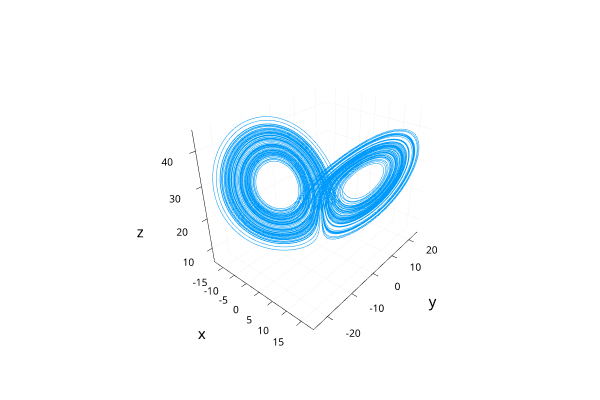
\includegraphics[width = 0.47\textwidth, trim={4.3cm, 1.9cm, 4.3cm, 3.5cm}, clip]{lorenz_actual_graph.png}
\end{figure}

I ran the SINDy algorithm on both data with noise of magnitude $\eta = 0.01$ and $\eta = 0.1$. Of interest is the system with $\eta = 0.1$ was only able to converge on a solution when the derivative was computed using the total-variation regularization derivative. 
For a function basis, I chose a basis comprised of all 7th-degree polynomial terms and all sines and cosines of the form $\sin{(ku_i)}$ and $\cos{(ku_i)}$ for all $\{u_i\} = \{x,y,z\}$ and integer $k$ from $1$ to $10$. This created a basis of $180$ possible functions. 
Further, the sparsification parameter was chosen to be $\lambda = 0.25$ with 10 iterations for sparse regression.
Integration of the input data was done over a timespan from $0$ to $100$ with $dt = 0.001$. 
The resulting systems from $\eta = 0.01$ are shown in Figure \ref{fig:lorenz_system_found_001} and the system resulting from $\eta = 0.1$ is shown in Figure \ref{fig:lorenz_system_found_01}. 

\begin{figure}[h]
	\caption{Discovered Lorenz system with noise $\eta = 0.01$}
	\label{fig:lorenz_system_found_001}

	\centering 
	\begin{minipage}{0.47\textwidth}
		\begin{center}
			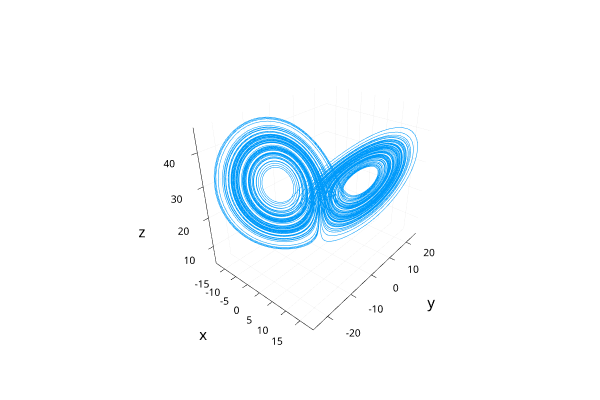
\includegraphics[width = \textwidth, trim={4.3cm, 1.9cm, 4.3cm, 3.5cm}, clip]{lorenz_found_001_normal.png}

			With standard derivative calculation
		\end{center}
	\end{minipage}%
	\begin{minipage}{0.47\textwidth}
		\begin{center}
			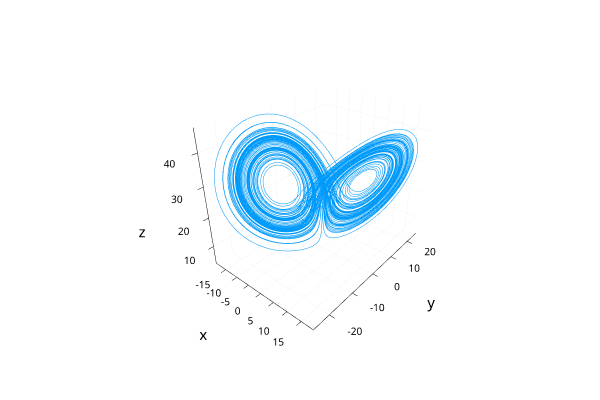
\includegraphics[width = \textwidth, trim={4.3cm, 1.9cm, 4.3cm, 3.5cm}, clip]{lorenz_found_001_tvdiff.png}

			With total-variation regularization derivative
		\end{center}
	\end{minipage}
\end{figure}	

\begin{figure}[h]
	\caption{Discovered Lorenz system with noise $\eta = 0.1$ and total-variation regularization differentiation}
	\label{fig:lorenz_system_found_01}

	\centering
	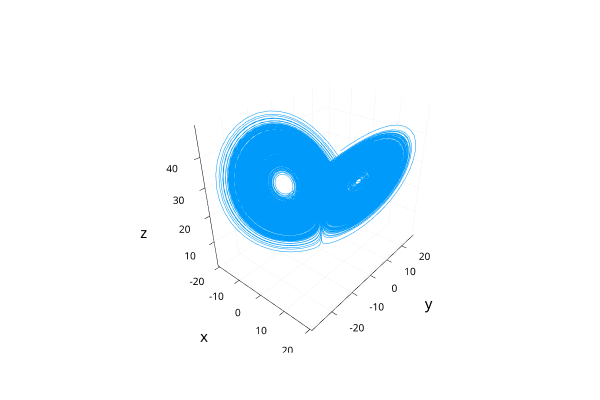
\includegraphics[width = 0.47\textwidth, trim={4.3cm, 1.9cm, 4.3cm, 3.5cm}, clip]{lorenz_found_01_tvdiff.png}
\end{figure}

We see that the SINDy algorithm was able to effectively capture the attracting dynamics present in the Lorenz system in all cases. Furthermore, for the standard derivative and noise $\eta = 0.01$, the discovered system had the form 
\begin{equation} \label{eq:found_lorenz_001}
	\begin{split}
		\dot x &= -9.982573809940325x + 9.999536628579511y, \\
	\dot y &= 27.573169299598813x - 0.8370109395705518y - 0.98935201514641xz, \\
	\dot z &= -2.660754272317803z + 0.9988807483584906xy.
	\end{split}
\end{equation}
Comparing this result to the actual system (Equation \ref{eq:lorenz}), we see that the discovered system has perfectly identified the polynomial terms in the system with coefficients that are almost identical. We see similar strength in identifying the system for $\eta = 0.01$ (Equation \ref{eq:found_lorenz_001_tv}) and $\eta = 0.1$ (Equation \ref{eq:found_lorenz_01_tv}) systems with total-variation regularization derivatives.
\begin{equation} \label{eq:found_lorenz_001_tv}
	\begin{split}
		\dot x &= -9.946417397865872x + 9.97621578174998y, \\
		\dot y &= 27.0485300793758x - 0.670689440675418y - 0.976667757332429xz, \\
		\dot z &= -2.6495215942228163z + 0.996381152512881xy.
	\end{split}
\end{equation}
\begin{equation} \label{eq:found_lorenz_01_tv}
	\begin{split}
		\dot x &= -9.805048724434341x + 9.835722669096466y, \\
		\dot y &= 25.92133086771059x - 0.433587521465246y - 0.946115512156319xz, \\
		\dot z &= -1.930341755171950 - 2.54324607967731z + 0.983562354075398xy.
	\end{split}
\end{equation}

We do see a forcing term introduced in the higher noise, $\eta = 0.1$, system for $\dot z$ which represents a term not present in actual system or the other two discovered systems. Though decreased performance is expected with higher noise. 

\subsection{Bifurcations: The Hopf normal form}
In addition to SINDy's ability to extract the system dynamics from the chaotic Lorenz attractor (\ref{sec:lorenz_results}), Section \ref{sec:SINDy} discussed how Brunton et al. discussed a modification to SINDy which would allow the detection of bifurcations in a system \cite{sindy}. 
Similar to the authors, I will demonstrate this using the Hopf normal form:
\begin{equation} \label{eq:hopf_normal}
	\begin{split}
		\dot x &= \mu x - \omega y - Ax(x^2 + y^2), \\
		\dot y &= \omega x +\mu y - Ay(x^2 + y^2).
	\end{split}
\end{equation} 
While $\mu$ is the bifurcation parameter and will be varried, I will take $\omega = A = 1$. In order for SINDy to discover the bifurcation in its system, we have to collect data over a range of $\mu$ values. 
In particular, I collected data for 16 values of $\mu$ between $-0.2$ and $0.55$, with a Hopf bifurcation occurring when $\mu = 0$. For negative values of $\mu$, I collected data with the initial condition $(x_0,y_0) = (2,0)$, while for positive values data was collected both for this initial condition and for $(x_0, y_0) = (0.01, 0)$ in order to capture the limit cycle behavior. 
Further, all collected data was given noise of magnitude $\eta = 0.005$. 

In order to account for multiple orbits worth of data, the derivatives for each orbit were calculated separately using the total-variation regularization derivative. Then, the $\mathbf X$ and $\mathbf {\dot X}$ matrices for all orbits were combined into a single data and derivative matrix. 
These could then be passed through SINDy as previously. For this example, a basis of all polynomials through 5th degree was used, with sparsity parameter $\lambda = 0.25$ and $10$ iterations of the sparse regression. Figure \ref{fig:discovered_hopf_0005} shows the discovered system as various values of $\mu$ and its ability to detect the Hopf bifurcation. 

\begin{figure}[h]
	\caption{Discovered Hopf bifurcation. Blue orbits start at $(x_0, y_0) = (2,0)$ and red orbits start at $(x_0, y_0) = (0.01, 0)$.}
	\label{fig:discovered_hopf_0005}

	\centering 

	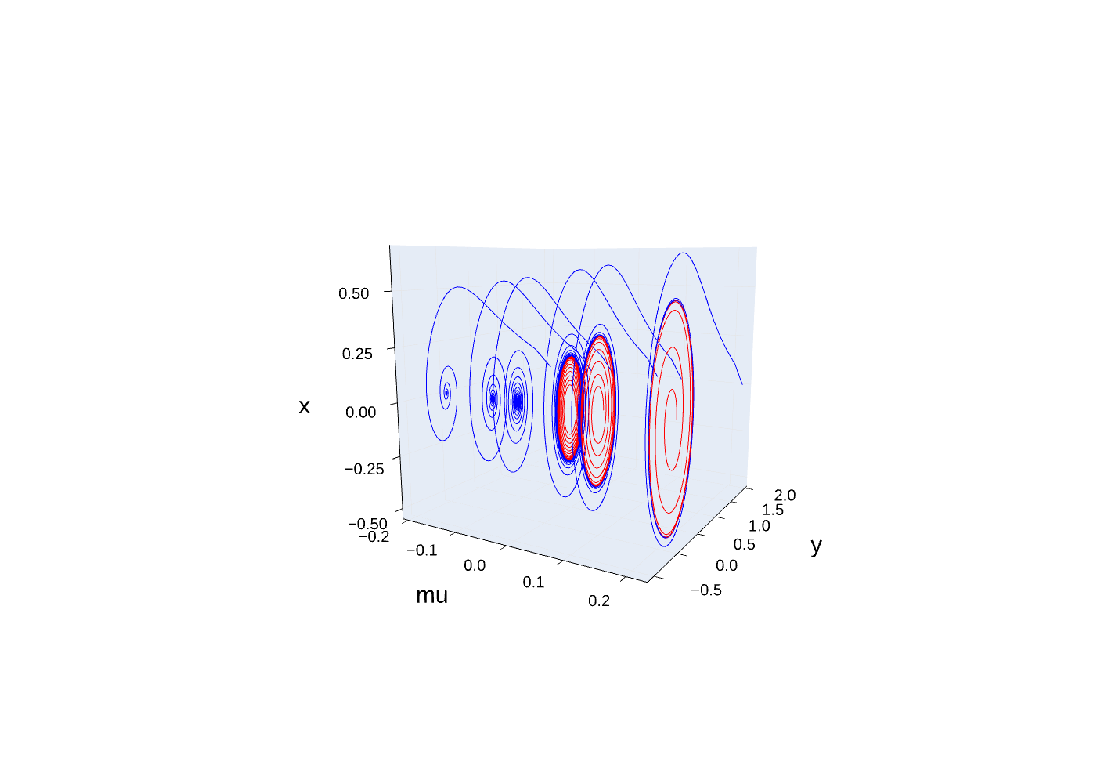
\includegraphics[width = 0.7\textwidth, trim={4.3cm, 1.9cm, 4.3cm, 3.5cm}, clip]{found_hopf_bifurcation_0005.pdf}
\end{figure}

Furthermore, SINDy found the system to be given by 

\begin{equation}\label{eq:discovered_hopf_0005}
	\begin{split}
		\dot x &= -0.9916y + 0.9314\mu x - 0.9178x^3 - 0.9178xy^2 - 0.3081x^4y, \\
		\dot y &= 0.9972x + 0.9926\mu y - 0.9811x^2y - 0.9814y^3.
	\end{split}
\end{equation}
Here we notice that barring the $-0.3081x^4y$ term in the equation for $\dot x$, the algorithm was able to identify the constants remarkably well and the nonlinear terms accurately. 
Though, its important to note that depending on the noise added to the system, the resulting system can be significantly worse. In particular, Equation \ref{eq:bad_discovered_hopf_0005} resulted from the same parameters but with different noise applied. 
\begin{equation}\label{eq:bad_discovered_hopf_0005}
	\begin{split}
		\dot x &= -0.9971y + 0.8704\mu x - 0.8617x^3 - 0.9177xy^2 + 0.9186\mu x^2 y  - 0.2853 xy^3 \\
		&\qquad - 0.9918 \mu x y^2 - 0.8546 x^4y + 1.2614 x^3y^2 - 1.0363 x^2y^3 + 1.0065 xy^4 \\ &\qquad + 0.5446\mu y^3 x, \\
		\dot y &= 0.9968x + 0.9930\mu y - 0.9807x^2y - 0.9822 y^3.
	\end{split}
\end{equation}
Interestingly, while $\dot y$ remained stable, $\dot x$ tends to me less stable. It is important to note, that while there are many additional higher-order polynomial terms, the qualatative behavior of the system is identical, still finding a Hopf bifurcation.

\section{Discussion} \label{sec:discussion}

% \section{}
% \label{sec:examples}

% \subsection{Sections}




% \begin{acknowledgments}

% We thank\dots

% \end{acknowledgments}

\newpage
\printbibliography

\end{document}